\section{Overview \& Design}
\label{design}

\begin{figure}[th!]
        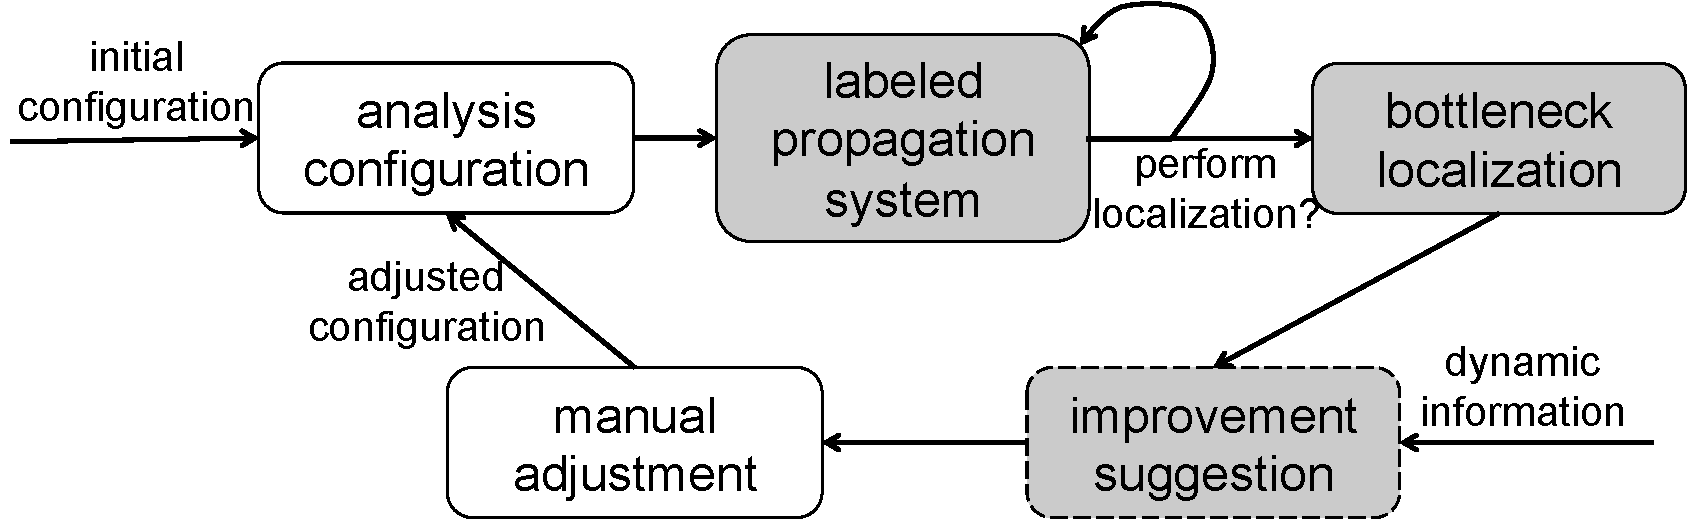
\includegraphics[width=0.9\columnwidth]{overview}
\caption{\textmd{Root cause localization process overview.}}
\label{fig:overview}
\end{figure}

{\bf Algorithms.}

\begin{algorithm}[th!]
\begin{algorithmic}[1]
{
\renewcommand{\algorithmicrequire}{\textbf{Input:}}
\renewcommand{\algorithmicensure}{\textbf{Output:}}
\REQUIRE {\tt config}: analysis configuration
\REQUIRE {\tt i}: evaluation interval
\ENSURE {\tt R}: set of root causes
\STATE {\tt sys} $\leftarrow$ initialize propagation system with {\tt Config}
\WHILE{({\tt c} $\leftarrow$ next constraint in {\tt sys}) != NULL //fixed-point has not been reached} 
%\STATE {\tt pts} $\leftarrow$ points-to propagation on {\tt c}
\FOR{each points-to assignment {\tt v1 = v2} from {\tt c}}
\STATE {\tt pts\textsubscript{v1}= pts\textsubscript{v1} $\bigcup$ pts\textsubscript{v2}} //points-to propagation
\STATE {\tt l\textsubscript{v1} = l\textsubscript{v1} $\bigcup$ l\textsubscript{v2} $\bigcup$ \{v2\}} //label propagation
\ENDFOR
\IF{{\tt (k $\leftarrow$ No. of evaluations) mod i = 0}}
\STATE  grow $\leftarrow$ points-to size growth in past {\tt i} evaluations
\IF{grow > threshold //to perform localization when the growth rate is high}
\STATE g $\leftarrow$ intermediate points-to graph with labels //do not require a complete graph
\FOR{each pointer key node {\tt n} in {\tt g}}
\STATE impact\textsubscript{n} $\leftarrow$ compute the impact of {\tt n} on {\tt g}
\ENDFOR
\STATE V $\leftarrow$ nodes with high impacts
\RETURN
\ENDIF
\ENDIF
\ENDWHILE
}
\end{algorithmic}
\caption{Root cause localization workflow.}
\label{alg:localization}
\end{algorithm}

\begin{algorithm}[th!]
\begin{algorithmic}[1]
{
\renewcommand{\algorithmicrequire}{\textbf{Input:}}
\renewcommand{\algorithmicensure}{\textbf{Output:}}
\REQUIRE {\tt R = \{r\textsubscript{1}, ..., r\textsubscript{n}\}}: root causes
\REQUIRE: {\tt t}: dynamic trace
\ENSURE {\tt <V, S>=\{(r\textsubscript{1}, s\textsubscript{1}),...,(r\textsubscript{n}, s\textsubscript{n})\}}: suggestions
\STATE G $\leftarrow$ taking {\tt t} as input, create a set of dynamic points-to graphs with different context sensitivity policies //some operations from Procedure 3 may be moved here
\FOR{each {\tt r\textsubscript{i}} $\in$ {\tt R}}
\STATE A\textsubscript{<r\textsubscript{i}, G>} $\leftarrow$ $\emptyset$ 
\FOR{each {\tt g\textsubscript{j}} $\in$ {\tt G}}
%\STATE |pts\textsubscript{(r, g)}| $\leftarrow$ query {\tt r}'s total points-to size in {\tt g}
%\STATE |cs\textsubscript{(r, g)}| $\leftarrow$ query number of calling contexts for {\tt r} in {\tt g}
\STATE a\textsubscript{<r\textsubscript{i}, g\textsubscript{j}>} $\leftarrow$ query {\tt r\textsubscript{i}}'s total points-to size in {\tt g\textsubscript{j}} and measure its accuracy corresponding to {\tt g\textsubscript{j}}'s context sensitivity policy
\STATE A\textsubscript{<r\textsubscript{i}, G>} = A\textsubscript{<r\textsubscript{i}, G>} $\bigcup$ \{a\textsubscript{<r\textsubscript{i}, g\textsubscript{j}>}\}
\ENDFOR
\STATE a\textsubscript{<r\textsubscript{i}, g>} $\leftarrow$ min(A\textsubscript{<r\textsubscript{i}, G>}) //pick the dynamic points-to graph on which r\textsubscript{i} is the most accurate
\STATE <V, S> = <V, S> $\bigcup$ \{<r\textsubscript{i}, g's context sensitivity>\}
\ENDFOR
}
\end{algorithmic}
\caption{Improvement suggestion workflow.}
\label{alg:suggestion}
\end{algorithm}

\subsection{Overview}

{\bf TODO: re-order the boxes in Figure \ref{fig:overview}.}

Figure \ref{fig:overview} shows an overview of the root cause localization process with the support of our automatic approaches. We first initialize the static analysis with an initial configuration in terms of context sensitivity, which experiences poor performance and/or precision behavior. The initial analysis is performed on the target program under a {\it labeled propagation system} which keeps track of the history of point-to propagations, labeling the origins of the points-to relations. Moreover, instead of waiting until the analysis achieves a fixed-point,\footnote{An analysis that experiences scalability issues on a program often cannot achieve the fixed-point within the time budget. This design allows us performing root cause localization on intermediate states during the points-to propagations.} we periodically pause the propagation system to evaluate the intermediate states. Heuristics are used to decide whether to perform {\it root cause localization} (i.e., when the abnormal behavior is observed); if not, the points-to propagations are resumed. The root cause localization identifies a set of variables and/or reference properties in the program as root causes of imprecision, using the points-to analysis history information collected by the labeled propagation system. The algorithm ranks the results in order of their impact to the overall analysis precision and therefore indicating their possibilities of being the root causes.

The optional {\it improvement suggestion} stage takes the localized root causes as inputs to automatically generate suggestions to improve the analysis with specialized context-sensitive analysis. The suggestions are based on the dynamic information. We collect in advance a dynamic trace of the program execution and compute dynamic points-to graphs based on the run-time information with pre-defined context sensitivity. Finally, a user (i.e., program analysis designer) may manually adjust the analysis configuration based on the localization results and/or the improvement suggestions. Furthermore, the analysis can be re-run under the adjusted configuration to observe if the performance and/or precision issues have been resolved. The same process may be performed multiple times to locate all the root causes and develop a specialized analysis configuration that would result in desired analysis performance and precision.

\subsection{Labeled Propagation System}

A propagation system for the points-to analysis solves the constraints to reach the fixed-point, propagating the points-to relations of the variables and reference properties in the program. A majority of the constraints that exist in the propagation system are assignments. For example, to process an invoke instruction, the generated constraints include assignments from the actual arguments to the formal parameters, from the callee's return values to the left-hand side variable of the invoke instruction, etc. The propagation system solves a constraint that assigns a variable {\tt v1} to another variable {\tt v2} by adding the points-to set of {\tt v1} to that of {\tt v2}. The results of such constraint propagations are therefore reflected in the points-to results. However, when the points-to set of a variable or a reference property is queried, the history information of the points-to relations is lost, which may originate from multiple transitive assignments. Such information is critical for identifying root causes because frequent assignments from an inaccurate points-to set may pollute the overall precision of the points-to analysis as indicated by the results in Figures \ref{fig:pts-growth} and \ref{fig:pts-distribution}.

In our labeled propagation system, each constraint that assigns the values of {\tt v1} to {\tt v2} results in not only the changes to {\tt v1}'s points-to relations but also a label {\tt v2} associated with the points-to set of {\tt v1} indicating the points-to relations of {\tt v1} were propagated from {\tt v2}. For example, the WALA's SSA IR represents the statement at line 5 in Figure \ref{fig:jquery-modified} as (a) {\tt v\textsubscript{tmp} = source[name]} and (b) {\tt target[name] = v\textsubscript{tmp}}, where {\tt v\textsubscript{tmp}}, {\tt source}, {\tt target} and {\tt name} are all local variables of the function.  For the property read instruction (a), the analysis would first query the points-to set of {\tt source}, {\tt P\textsubscript{source}}, and the points-to set of {\tt name}, {\tt P\textsubscript{name}}. The pairs of each element in {\tt P\textsubscript{source}} and {\tt P\textsubscript{name}} (e.g., {\tt p\textsubscript{source\_i}.p\textsubscript{name\_j}}) are returned as the results of looking up the reference properties of {\tt source[name]}. Note that the values of {\tt name} iterate over all the property names of {\tt source}, which in practice are the large set of the function names loaded in {\it jQuery}. It eventually results in a large points-to set for {\tt v\textsubscript{tmp}} due to multiple assignments from various reference properties and we keep all these reference properties (e.g., {\tt p\textsubscript{source\_i}.p\textsubscript{name\_j}}) as labels for the points-to set of {\tt v\textsubscript{tmp}}. For the property write instruction (b), the analysis similarly looks up the reference properties of {\tt target[name]} (e.g., {\tt p\textsubscript{target\_i}.p\textsubscript{name\_j}}) and adds the points-to relations of {\tt v\textsubscript{tmp}} to each of these reference properties, resulting in overly-approximated points-to set for each function name of {\it jQuery}. We keep both {\tt v\textsubscript{tmp}} and the transitively existing labels from {\tt v\textsubscript{tmp}} (e.g., {\tt p\textsubscript{source\_i}.p\textsubscript{name\_j}}) for the points-to set of each reference property of {\tt target[name]}.

More interestingly, in addition to tracking the set of labels that are immediately or transitively propagated to the points-to set of a variable or a reference property, we generate a {\it propagation-history graph} for the points-to set of each variable and reference property, which represents the hierarchical information of the points-to propagation history. Intuitively, a node in the propagation-history graph is a variable or a reference property that has an impact on the specific points-to set. An edge from a node {\tt n\textsubscript{1}} to another node {\tt n\textsubscript{2}} represents that the points-to set of {\tt n\textsubscript{2}} was explicitly added to that of {\tt n\textsubscript{1}}. The entry points of the graph are the variables and/or reference properties whose points-to sets are directly propagated into the corresponding points-to set. For the same example in Figure \ref{fig:jquery-modified}, the propagation-history graph for the points-to set of {\tt v\textsubscript{tmp}} consists of all the reference properties of {\tt source[name]} as entry points. {\tt v\textsubscript{tmp}} is the entry point of the propagation-history graph for the points-to set of each reference property of {\tt target[name]} (e.g., {\tt p\textsubscript{target\_i}.p\textsubscript{name\_j}}), while there also are edges from {\tt v\textsubscript{tmp}} to the properties of {\tt source[name]}.

\subsection{Root Cause Localization}

\begin{figure}[th!]
        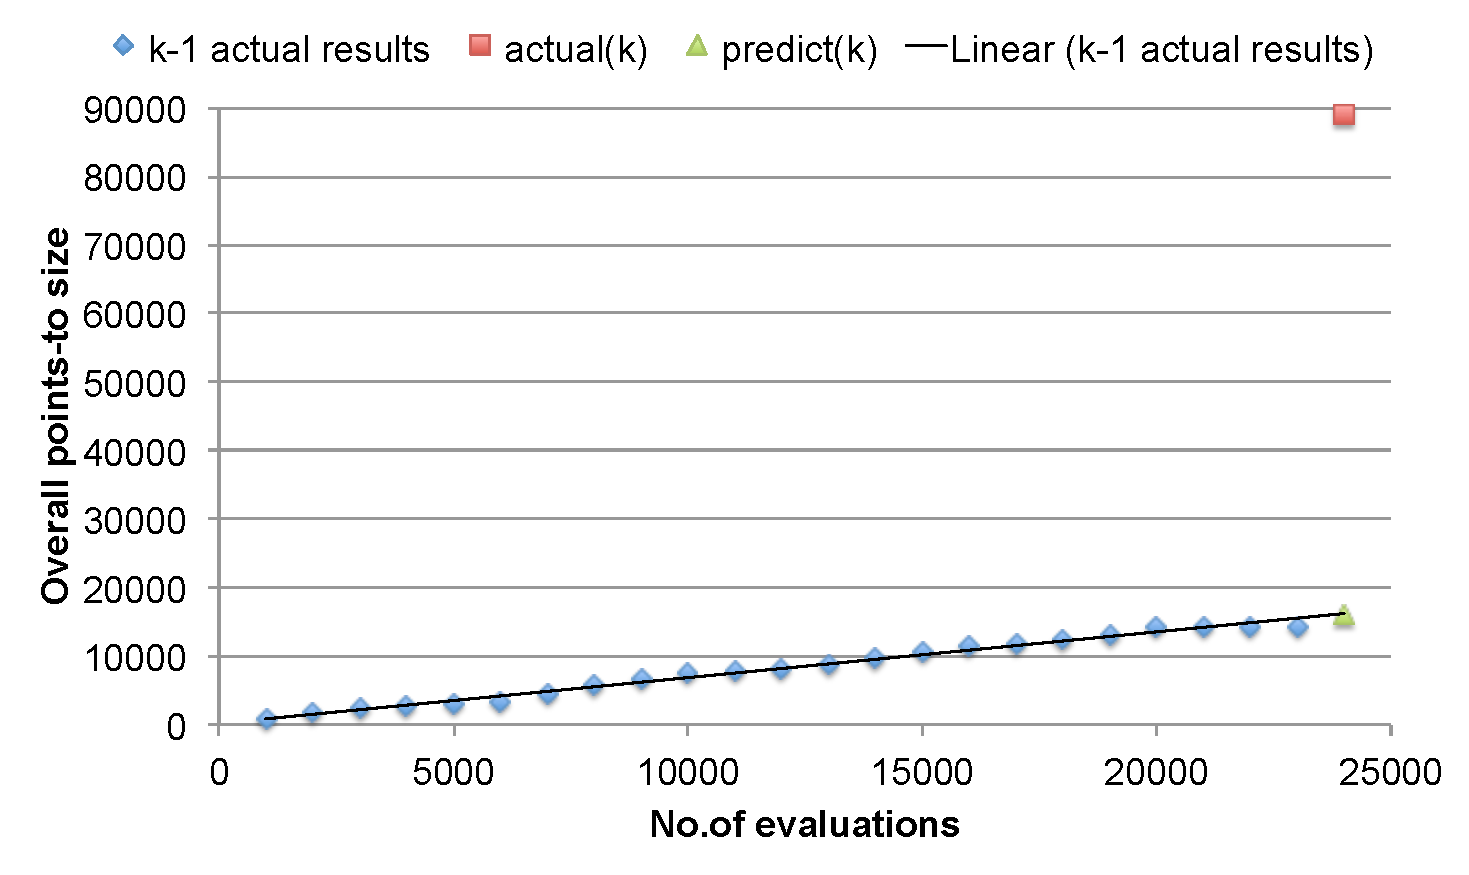
\includegraphics[width=\columnwidth]{linear}
\caption{\textmd{Prediction via linear regression.}}
\label{fig:linear}
\end{figure}

During the process, the labeled propagation system is paused every {\tt n} evaluations. We use the intermediate states to decide whether root cause localization is performed. We count the total number of points-to relations (i.e., edges) in the intermediate points-to graph for the {\tt k\textsubscript{th}} pause (i.e., after {\tt n$\times$k} evaluations), {\tt actual(k)}. We compare the value of {\tt actual(k)} with the value of {\tt predict(k)} to decide on whether to perform root cause localization. Using intermediate results from the previous {\tt k-1} pauses, we perform a simple linear regression to find the fitted line {\tt y = intercept + slope $\times$ x}, where {\tt x} is the number of evaluations and {\tt y} is the total number of points-to relations. Therefore, the number of points-to relations of the {\tt k\textsubscript{th}} pause can be predicted: {\tt predict(k) = intercept + slope $\times$ kn}. If {\tt actual(k) > 110\% $\times$ predict(k)}, we decide to perform the root cause localization at the {\tt k\textsubscript{th}} pause; otherwise, we continue the points-to analysis under the labeled propagation system. Figure \ref{fig:linear} shows this prediction model running the 0-1-CFA analysis on a {\it jQuery} application. The analysis is paused every 1000 evaluations and the fitted line in Figure \ref{fig:linear} is calculated from the results of the first 23 pauses (i.e., 1000 to 23,000 evaluations). The predicted total points-to edges at the 24,000 evaluations is 16,234, while {\tt actual(24)} is 88,857, significantly passing the threshold to perform the root cause localization. This prediction model can capture the ``jump'' period of the points-to analysis shown in Figure \ref{fig:pts-growth} and is important for accurately localizing the root causes. If the localization is performed too early, the overly-approximated results may have not surfaced. If the localization is performed late during the analysis, the overly-approximated results of the root causes may have polluted a large portion of the overall points-to results, making it difficult to identify the root causes of imprecision. Moreover, the evaluation interval to pause the analysis, {\tt n}, as well as the decision threshold may be tuned based on the budget and goals of root cause localization.

%During the progress, the label propagation system is paused periodically. The intermediate results are used to decide whether bottleneck localization is performed, using the predicted value of linear regression. A linear regression is predicted based on the {\tt k-1} pauses. If the actual value of the {\tt k}'s pause is greater than 110\% of the predicted value, we determine that the analysis may have entered the ``jump" period shown in Figure \ref{fig:pts-growth} and the bottleneck localization is performed.

When performing root cause localization, we use the intermediate points-to graph and the associated labels to identify possible root causes. For each variable or reference property {\tt v}, we count (i) its points-to size, {\tt |P\textsubscript{v}|}, and (ii) its number of occurrences as labels in the points-to sets of other variables and/or reference properties, {\tt |L\textsubscript{v}|}. {\tt |L\textsubscript{v}|} measures how widely {\tt v} reaches within the propagation system and {\tt |P\textsubscript{v}|} measures if the impact of its wide reach is significant. We therefore use the score {\tt S\textsubscript{v}=|P\textsubscript{v}|$\times$|L\textsubscript{v}|} as a measurement of the possibility of {\tt v} being the root cause. The root cause localization stage reports a set of variables as root causes in descending order of their scores. For example, {\tt v\textsubscript{tmp}}, the result of the property read instruction at line 5 in Figure \ref{fig:jquery-modified}, has a extremely high score (73,950) with {\tt |P\textsubscript{v\textsubscript{tmp}}|=150} and {\tt |L\textsubscript{v\textsubscript{tmp}}|=493} when the root cause localization is performed after the 24,000 evaluations. Its score is 75 times higher than the variable with the second highest score (990), making it the only candidate as the root cause of imprecision of 0-1-CFA analysis for this {\it jQuery} application. We report the variables and/or reference properties whose scores are at least 50\% the highest score as {\it suspicious root causes}.

%We then assign score to each variable and/or reference property by calculating (i) $\times$ (2). The higher score indicates the variable is more likely to be analysis bottlenecks. We report the variables with scores great than half of the one with the highest scores.

\subsection{Improvement Suggestion}

We have discussed the approaches that automatically identifies the root causes of imprecision. A user may manually adjust the analysis to improve the analysis precision on these root causes. More automatic support on suggesting possible analysis configurations will further assist in improving the analysis precision on the program. We present automatic improvement suggestion in terms of a specialized context-sensitive analysis.

First, the target program is executed to collect a dynamic trace, recording the following run-time information in order of occurrence: (i) function enters and exits, (ii) invocations, and (iii) property reads and writes. At a property read or write instruction we record (i) the instruction location in the program, (ii) the allocation site (in terms of the program location) of the base object, (iii) the property name, and (iv) the allocation site of the value if it is a reference object or the type of the value if it is primitive. At an invoke instruction we record (i) the location of the call site, (ii) the location of the target function, (iii) the allocation site of the receiver object, and (iv) the allocation sites and/or the types of the actual arguments. Second, dynamic points-to graphs based on the dynamic trace are generated under various kinds of context sensitivity. Procedure \ref{alg:dyn-pts} shows the algorithm that produces a dynamic points-to graph with respect to a specific context-sensitive analysis (e.g., 1-CFA, argument-sensitive or context-insensitive analysis). It takes the dynamic trace, {\tt Trace}, and the kind of context sensitivity, {\tt CS}, as inputs. The algorithm iterates through all the instructions recorded in the dynamic trace. For each instruction {\tt i}, the algorithm examines its kind. If it is an invoke instruction, at line 5, the call site and the argument are pushed into the call stack, {\tt Stack}. If it exits a function, the top element of {\tt Stack} is removed  at line 7. If it is a property read or write instruction, at lines 9 to 15, depending on the input context sensitivity, the calling context, {\tt Context}, is determined by the call site and the argument from the top element of {\tt Stack} for 1-CFA and argument-sensitive analysis, respectively; the calling context is {\it everywhere} for context-insensitive analysis. In the dynamic points-to graph, a variable is represented by (i) the location of the instruction, (ii) the part of the instruction (i.e., base, property or value), and (iii) the calling context. At lines 16 to 18, the object allocation site, represented by program location, of each part of the instruction collected at runtime is assigned to the corresponding variable node in the dynamic points-to graph. Note that this algorithm is general in that various dynamic points-to graphs that can be generated under different context sensitivity.
%The ultimate goal of our proposed approach is to improve the performance and/or precision of the analysis on the program. The identified bottlenecks are the program constructs 

\newcommand{\SWITCH}[1]{\STATE \textbf{switch} (#1) \begin{ALC@g}}
\newcommand{\ENDSWITCH}{\end{ALC@g} \STATE \textbf{end switch}}
\newcommand{\CASE}[1]{\STATE \textbf{case} #1\textbf{:} \begin{ALC@g}}
\newcommand{\ENDCASE}{\end{ALC@g}}
\newcommand{\CASELINE}[1]{\STATE \textbf{case} #1\textbf{:} \begin{ALC@g}}
\newcommand{\DEFAULT}{\STATE \textbf{default:} \begin{ALC@g}}
\newcommand{\ENDDEFAULT}{\end{ALC@g}}
\newcommand{\DEFAULTLINE}[1]{\STATE \textbf{default:} }

\begin{algorithm}[th!]
\floatname{algorithm}{Procedure}
\begin{algorithmic}[1]
{
\renewcommand{\algorithmicrequire}{\textbf{Input:}}
\renewcommand{\algorithmicensure}{\textbf{Output:}}
\REQUIRE {\tt Trace}: dynamic trace; {\tt CS}: context sensitivity
\ENSURE {\tt G}: dynamic points-to graph
\STATE {\tt Stack = empty}
\WHILE{{\tt (i = next(Trace)) != NULL}}
\SWITCH {{\tt kindOf i}}
\CASE {{\tt INVOKE}}
 \STATE  {\tt Stack.push(Pair(i\textsubscript{callsite}, i\textsubscript{arg1}))}
 \ENDCASE
\CASELINE {{\tt FEXIT}}
 \STATE  {\tt Stack.pop}
 \ENDCASE
  \CASELINE {{\tt PREAD || PWRITE}}
  \IF{{\tt CS = 1-CFA}}
\STATE {\tt Context = S.top().fst}
\ELSIF{{\tt CS = argument-sens}}
 \STATE {\tt Context = S.top().snd}
 \ELSIF{{\tt CS = context-insens}}
 \STATE {\tt Context = everywhere}
\ENDIF
\STATE {\tt G\textsubscript{(i\textsubscript{loc},base,Context)} $\rightarrow$ i\textsubscript{base}}
\STATE {\tt G\textsubscript{(i\textsubscript{loc},property,Context)} $\rightarrow$ i\textsubscript{property}}
\STATE {\tt G\textsubscript{(i\textsubscript{loc},value,Context)} $\rightarrow$ i\textsubscript{value}}
 \ENDCASE
\ENDSWITCH
\ENDWHILE
}
\end{algorithmic}
\caption{Dynamic points-to graph generation.}
\label{alg:dyn-pts}
\end{algorithm}

Now that we have obtained the dynamic points-to graphs under different context-sensitive analyses (i.e., 1-CFA, argument-sensitive and context-insensitive). For a variable {\tt v} that is identified as a root cause, we locate its corresponding nodes via its program location in each dynamic points-to graph and collect (i) the number of calling contexts associated with {\tt v}, {\tt |CS|}, and (ii) the sum of points-to sizes under all calling contexts, {\tt $\sum$|P\textsubscript{v}|}. We then count {\tt D\textsubscript{v} = $\sum|P\textsubscript{v}|\over |CS|$}, the average dynamic points-to size per calling context, to measure the accuracy of the points-to relations of {\tt v} under the specific context sensitivity. The context sensitivity under which {\tt D\textsubscript{v}} is the smallest is chosen for the function that contains {\tt v} as the improvement suggestion.

{\bf TODO: discussions on why using dynamic information and the impact of its incompleteness.} 